% Lecture notes: physics and numerical methods of the LIONS benchmarks.
% Build: uv run --group bench --with pandas python docs/lecture/figures.py
%        cd docs/lecture && latexmk -lualatex -outdir=out lecture.tex
\documentclass[11pt,a4paper]{report}
\usepackage{fontspec}
\usepackage{unicode-math}
\usepackage[margin=2.5cm]{geometry}
\usepackage{amsmath}
\usepackage{graphicx}
\usepackage{booktabs}
\usepackage{siunitx}
\usepackage{tikz}
\usetikzlibrary{arrows.meta,calc,decorations.pathreplacing}
\usepackage[numbers,sort&compress]{natbib}
\usepackage{xcolor}
\usepackage[colorlinks,linkcolor=blue!50!black,citecolor=green!40!black,urlcolor=blue!50!black]{hyperref}
\usepackage[capitalise,noabbrev]{cleveref}
\usepackage{caption}
\usepackage[htt]{hyphenat}
\captionsetup{font=small,labelfont=bf}
\sisetup{exponent-product=\times,round-mode=none}

\graphicspath{{gen/}}
\input{gen/numbers.tex}
\input{gen/code.tex}

\newcommand{\thirddeg}{$1/3^\circ$}
\newcommand{\dd}{\mathrm{d}}
\newcommand{\e}{\mathrm{e}}
\newcommand{\vect}[1]{\symbf{#1}}
\newcommand{\Qr}{Q_r}
\newcommand{\Qz}{Q_z}
\newcommand{\unverified}{\textsf{[UNVERIFIED]}}
\newenvironment{reading}{\par\medskip\noindent\textbf{Reading.}\ }{\par\medskip}

\title{Tracking ions in sector cyclotrons:\\ fields, integrators and verification\\[1ex]
  \large Lecture notes on the LIONS benchmarks (Phase 5)}
\author{Benchmark work by A.~Ghribi, with the LIONS Python port by O.~Kamalou}
\date{Code \CodeVersion, 2026-11-01}

\begin{document}
\maketitle

\begin{center}
\fbox{\parbox{0.85\textwidth}{\small
\textbf{Internal document.}
Chapters~\ref{ch:results} and \ref{ch:options} contain results computed from the PSI Ring cyclotron field map and FIXPO
reference orbits published in the OPALX-project repositories without a licence.
This document is not to be redistributed outside the LIONS/CIME team until PSI grants permission.
Every number in the text, tables and figures is produced by \nolinkurl{docs/lecture/figures.py} from the benchmark
tables listed in \cref{app:provenance}; the few values quoted from the design note \nolinkurl{benchmarks/DESIGN.md}
are marked as such.}}
\end{center}

\tableofcontents

\chapter{Introduction}\label{ch:intro}

LIONS tracks ions through a sector cyclotron, from the central region to extraction.
It integrates the relativistic Lorentz equation with a Boris push in a static median-plane magnetic map and in RF
electric potential maps of the dees.
The code was written in Fortran~90 by P.~Bertrand (GANIL) for the CIME cyclotron, and ported to Python by
O.~Kamalou.
The Python port keeps the Fortran results bit for bit on the default path: \nolinkurl{tests/test_fortran.py} compares
it with a \texttt{gfortran} build compiled with \texttt{-ffp-contract=off}.

These notes explain the physics and the numerical methods behind the Phase~5 benchmarks.
The benchmarks ask five questions (\nolinkurl{benchmarks/DESIGN.md}, section~1):
\begin{enumerate}
\item[Q1] Do LIONS, OPAL-cycl and RF-Track agree on the same fields at the same time step?
\item[Q2] Is the LIONS one-turn map symplectic, and how does it compare with OPAL and RF-Track integrators?
\item[Q3] Can the LIONS core be made differentiable at an acceptable cost?
\item[Q4] Do the codes agree on acceleration through the dee gaps?
\item[Q5] Does the extracted beam survive the conversion to Xsuite and Cheetah?
\end{enumerate}
Q1 to Q3 have answers in these notes.
Q4 (case C) and Q5 (case F) were not run: case C waits for the CIME maps, and case F has nothing after extraction to compare yet.

\section*{Plan}
\Cref{ch:motion,ch:fields} cover the physics: motion in a cyclotron, focusing, and fields in the median plane.
\Cref{ch:interpolation,ch:integrators,ch:orbits} cover the numerical methods: field interpolation, integrators, closed
orbits and tunes.
\Cref{ch:method} states the verification method.
\Cref{ch:results} gives the benchmark results (cases A, B, D, G).
\Cref{ch:options} covers the field-model options added to LIONS (case H).
\Cref{ch:differentiable} covers the differentiable port (cases E, E2).
\Cref{ch:open} lists what is open.

\section*{Conventions}
Positions in \si{m}, time in \si{s}, fields in \si{T} and \si{V/m}.
Momenta are normalised, $p = \beta\gamma = |\vect p|/(m_0 c)$, as in LIONS.
$(r,\theta,z)$ are cylindrical coordinates with $z$ normal to the median plane, and $\theta$ is measured from $x$ towards $y$.
In LIONS a positive ion turns counter-clockwise ($\theta$ increasing) when $B_z<0$.
Tunes are folded into $[0,0.5]$ when compared, because the trace of the one-turn matrix only fixes the fractional
tune modulo this symmetry (\cref{ch:orbits}).
``Relative error'' always means the error divided by the reference value.

\chapter{Motion in a cyclotron}\label{ch:motion}

\section{Lorentz equation}
A particle of rest mass $m_0$ and charge $q$ obeys
\begin{equation}
\frac{\dd \vect P}{\dd t} = q\left(\vect E + \vect v\times\vect B\right),\qquad
\vect P = \gamma m_0 \vect v,\qquad \gamma = \sqrt{1+p^2},\qquad \vect p = \vect P/(m_0c).
\label{eq:lorentz}
\end{equation}
In a static magnetic field $\vect v\cdot(\vect v\times\vect B)=0$, so $|\vect p|$ and $\gamma$ are constants of the
motion.
This exact invariant is the first test of any integrator (case A, \cref{sec:caseA}).

In a uniform field $\vect B = B\hat z$ the motion in the plane is a circle of radius $\rho$ at angular frequency
$\omega$:
\begin{equation}
\rho = \frac{P}{|q B|} = \frac{m_0 c\, p}{|qB|},\qquad \omega = \frac{|q B|}{\gamma m_0},
\qquad B\rho = \frac{P}{q}.
\label{eq:cyclotron}
\end{equation}
The non-relativistic frequency $|qB|/m_0$ does not depend on the energy.
This is the principle of the cyclotron: an RF voltage at a harmonic $h$ of $\omega$ accelerates the ion at each gap
crossing while the orbit radius grows.

The direction of rotation follows from the force.
For counter-clockwise motion $\vect v = v\hat\theta$, and $q\,\vect v\times\vect B = q v B_z\,\hat\theta\times\hat z
= q v B_z\,\hat r$.
The force must point to the centre, so $qB_z<0$: in LIONS a positive ion turns counter-clockwise in $B_z<0$.

\section{Isochronism}
With relativity, $\omega = |qB|/(\gamma m_0)$ falls as the energy grows.
To keep the revolution frequency at $\omega_0$, the azimuthally averaged field $\bar B(r)$ must grow with $\gamma$.
On an orbit of radius $r$, $v = \omega_0 r$, so $\beta = r/r_\infty$ with $r_\infty = c/\omega_0$, and
\begin{equation}
\bar B(r) = \gamma(r)\, B_0 = \frac{B_0}{\sqrt{1-r^2/r_\infty^2}},\qquad B_0 = \frac{m_0\omega_0}{|q|}.
\label{eq:isochronous}
\end{equation}
Define the field index
\begin{equation}
k = \frac{r}{\bar B}\frac{\dd \bar B}{\dd r}.
\end{equation}
From \cref{eq:isochronous}, $\dd\gamma/\dd r = \gamma^3 r/r_\infty^2$, hence
\begin{equation}
k = \frac{r}{\gamma}\,\frac{\gamma^3 r}{r_\infty^2} = \gamma^2\beta^2 = \gamma^2-1 .
\label{eq:k-isochronous}
\end{equation}
An isochronous field grows with radius ($k>0$).
In a weak-focusing machine (\cref{sec:weak}) this defocuses vertically, and the cyclotron must recover vertical
focusing elsewhere: from the azimuthal variation of the field.

The FROM\_ORBIT maps used in case G (\cref{sec:caseG1}) are isochronous by construction, with $r_\infty$ = \SI{5}{m}
(3-sector example) and \SI{28}{m} (10-sector example) \cite{planche2019}.

\section{Linear motion near a circular orbit}\label{sec:weak}
Take an azimuthally symmetric field $B_z(r)$ in the median plane, with $n = -k = -(r/B)\,\dd B/\dd r$ evaluated on the
reference orbit of radius $\rho$.
Use $\theta$ as the independent variable and write $r = \rho + x$.
To first order in $x$ and $z$, the radial and vertical motions decouple:
\begin{equation}
\frac{\dd^2 x}{\dd\theta^2} + (1-n)\,x = 0,\qquad \frac{\dd^2 z}{\dd\theta^2} + n\,z = 0 .
\end{equation}
The radial term $1$ is the geometric focusing of the circle; the gradient term $\mp n$ comes from the radial derivative
of $B_z$ and, through $\nabla\times\vect B = 0$, from $B_r = z\,\partial B_z/\partial r$ (\cref{ch:fields}).
The number of betatron oscillations per turn, the tunes, are
\begin{equation}
\Qr = \sqrt{1-n} = \sqrt{1+k},\qquad \Qz = \sqrt{n} = \sqrt{-k} .
\label{eq:weak-tunes}
\end{equation}
Both planes are stable only for $0<n<1$ \cite{kerst1941}.
This is the field used in case B0 (\cref{sec:caseB0}), where \cref{eq:weak-tunes} gives the exact reference tunes.

In an isochronous field, $k = \gamma^2-1 > 0$, so $\Qr\simeq\gamma$ and $\Qz^2<0$: the vertical motion is unstable without
another focusing mechanism.

\section{Sector focusing}
Thomas \cite{thomas1938} showed that an azimuthally varying field (alternating hills and valleys) gives vertical
focusing.
The orbit is no longer a circle: it is scalloped, and it crosses the hill edges at an angle.
At each crossing, the azimuthal field component $B_\theta = (z/r)\,\partial B_z/\partial\theta$ combines with the radial
velocity component to give a vertical force.
Averaged over a turn, this force is focusing.
Spiral sector edges add an alternating-gradient focusing in the sense of Courant and Snyder \cite{courant1958}.
They are used in FFAG accelerators \cite{symon1956}; the PSI Ring map of case G2 has eight spiral sectors
\cite{grillenberger2021}.

Define the flutter of a field with $N$ sectors,
\begin{equation}
F = \frac{\langle (B-\bar B)^2\rangle}{\bar B^2},
\end{equation}
where $\langle\cdot\rangle$ is the azimuthal average on a circle, and the spiral angle $\xi$ of the hill edges.
In the smooth approximation the tunes are \cite{zaremba2017}
\begin{align}
\Qz^2 &\simeq -k + \frac{N^2}{N^2-1}\,F\,(1+2\tan^2\xi), \label{eq:smooth-qz}\\
\Qr^2 &\simeq 1 + k + \frac{3N^2}{(N^2-1)(N^2-4)}\,F\,(1+\tan^2\xi). \label{eq:smooth-qr}
\end{align}
(The source writes the field index with the opposite sign; \cref{eq:smooth-qz,eq:smooth-qr} use $k$ as defined above.)
Two consequences shape the benchmarks.
First, $\Qr\simeq\gamma$ in an isochronous cyclotron: $\Qr$ crosses integer and half-integer values as the energy grows.
In the FIXPO reference tunes of the PSI Ring (case G2), $\Qr$ crosses $1.5$ between 386 and \SI{430}{MeV}, where the
tune formula of \cref{ch:orbits} is ill-conditioned.
Second, at low energy $\Qr$ is close to $1$, which makes the closed orbit sensitive to small field errors
(\cref{sec:conditioning}).

\paragraph{Check on case B.}
The case B field is $B_z = B_0(1+\epsilon\cos 4\theta)$ with $\epsilon = 0.3$, $k=0$ and radial sector edges.
Its flutter is $F = \epsilon^2/2 = \BFlutter$.
\Cref{eq:smooth-qz,eq:smooth-qr} give $\Qz = \BSmoothQz$ and a fractional $\Qr$ of $\BSmoothQrFrac$.
LIONS at 1440 steps per turn finds $\Qz = \BLionsQz$ and a fractional $\Qr$ of $\BLionsQr$ (1~MeV protons).
The smooth approximation is good to the third digit here, because $\epsilon$ is small.

\section{What LIONS models}
LIONS integrates \cref{eq:lorentz} for many particles, with
\begin{itemize}
\item a median-plane magnetic map $B_z(r,\theta)$ with its first-order off-plane expansion (\cref{ch:fields});
\item two dees, each described by an electrostatic potential map scaled by $V\cos(\omega_{\rm rf}t+\phi)$: a Cartesian map in the
central region, and a normalised single-gap map in the outer region;
\item extraction elements: electrostatic deflectors, gradient dipoles and recording grids;
\item an initial bunch drawn from a $6\times6$ sigma matrix, and a vertical sorter.
\end{itemize}
It does not model space charge, a full 3D magnetic map, misalignments or charge exchange.
The cases in these notes use the static magnetic part only: no RF and no extraction.
LIONS was first described by Bertrand for the CIME injection studies \cite{bertrand1995,bertrand1998}; CIME is the
cyclotron of the SPIRAL facility at GANIL \cite{bourgarel1998}.

\chapter{Magnetic fields in the median plane}\label{ch:fields}

\section{Expansion off the median plane}
In the beam region the static field satisfies $\nabla\times\vect B = 0$ and $\nabla\cdot\vect B = 0$.
So $\vect B = \nabla\Phi$ with $\nabla^2\Phi = 0$.
A cyclotron magnet is symmetric about the median plane $z=0$: $B_z$ is even in $z$, $B_r$ and $B_\theta$ are odd.
Then $\Phi$ is odd in $z$:
\begin{equation}
\Phi(r,\theta,z) = z\,B(r,\theta) + z^3 a_3(r,\theta) + O(z^5),
\end{equation}
where $B(r,\theta)$ is the median-plane field.
Write $\nabla_\perp^2 = \partial_r^2 + r^{-1}\partial_r + r^{-2}\partial_\theta^2$.
Laplace's equation, order by order in $z$, gives $6a_3 + \nabla_\perp^2 B = 0$.
Differentiating $\Phi$:
\begin{align}
B_z &= B - \frac{z^2}{2}\,\nabla_\perp^2 B + O(z^4),\label{eq:bz-expansion}\\
B_r &= z\,\frac{\partial B}{\partial r} + O(z^3),\qquad
B_\theta = \frac{z}{r}\,\frac{\partial B}{\partial\theta} + O(z^3).\label{eq:br-expansion}
\end{align}
In Cartesian components, $B_x = z\,\partial B/\partial x$ and $B_y = z\,\partial B/\partial y$ to the same order.
A median-plane map of $B$ and its first derivatives therefore fixes the field to first order in $z$, which is all that
linear vertical motion needs.

\paragraph{The truncated field.}
LIONS and OPAL keep \cref{eq:br-expansion} and $B_z = B$ (OPAL), or $B_z = B - (z^2/2)\,D$ with a map $D$ (LIONS).
Every benchmark here sets $D = 0$, as OPAL does.
With $D = 0$ the truncated field is exactly curl-free: for example $\partial_z B_r - \partial_r B_z = \partial_r B - \partial_r B = 0$,
and the other two components vanish the same way.
(With $D\ne0$, $(\nabla\times\vect B)_r = -(z^2/2r)\,\partial_\theta D$ and $(\nabla\times\vect B)_\theta = (z^2/2)\,\partial_r D$.)
It is not divergence-free:
\begin{equation}
\nabla\cdot\vect B = \frac{1}{r}\partial_r(r B_r) + \frac{1}{r}\partial_\theta B_\theta + \partial_z B_z
= z\,\nabla_\perp^2 B \quad (D = 0).
\end{equation}
The missing $-(z^2/2)\nabla_\perp^2B$ term in $B_z$ is what cancels it.
For the linear tunes this does not matter, because the term is second order in $z$.
For long-term invariants at finite $z$ it does.
A divergent field has no vector potential, so the motion off the plane is not Hamiltonian and the canonical angular
momentum is no longer an invariant ($|\vect p|$ still is, as for any magnetic field).
The Lorentz flow even keeps preserving phase-space volume, since $\partial_{\vect p}\cdot(\vect v\times\vect B) = 0$ for any
$\vect B$: a determinant test cannot detect the divergence.
Case D2 (\cref{sec:caseD}) therefore uses planar motion only.

\paragraph{The $D$ map in LIONS.}
The LIONS map file stores a second block after $B_z$, documented as $\partial^2B_z/\partial r^2$, which multiplies $-z^2/2$.
\Cref{eq:bz-expansion} shows that it must hold the transverse Laplacian $\nabla_\perp^2B$; with that choice and the
truncated $B_r$, $B_\theta$, $\nabla\cdot\vect B = 0$ exactly, at the price of a curl of order $z^2$.
The field-harmonic routine of LIONS adds the Laplacian of the harmonic polynomial to it, consistent with
\cref{eq:bz-expansion}.
What the CIME map files contain in that column has not been checked here.

\section{Map formats and conventions}
Three formats appear in the benchmarks.
Each conversion goes through one function (\nolinkurl{benchmarks/convert.py} or a case driver), validated on a
reference case.
The conventions below were settled from the files and the OPAL source, then confirmed by a run (\texttt{DESIGN.md},
sections 3, 7 and 21).

\begin{description}
\item[LIONS.] An $(r,\theta)$ grid over \SI{360}{\degree}, endpoint included, with $B_z$, $D$, $\partial B/\partial x$ and
$\partial B/\partial y$ in \si{T} and \si{T/m}.
The Python port accepts 250 radii and 1081 azimuths (the Fortran: 721 azimuths); 1081 columns at \thirddeg{} is the
native PSI resolution.
$B_z<0$ for counter-clockwise positive ions.
\item[OPAL \texttt{CARBONCYCL}.] Header $r_{\min}$ [\si{mm}], $\Delta r$ [\si{mm}], $\theta_{\min}$ [\si{\degree}],
$\Delta\theta$ [\si{\degree}], then $B_z$ in \si{kG} on $n_r\times n_\theta$ nodes, with no \SI{360}{\degree} endpoint.
Values are read with \texttt{fscanf("\%16lE")}: at most 16 characters per value, so a longer number is silently split
in two.
A $+\SI{10}{kG}$ map gives $B_z = \SI{-1}{T}$ inside OPAL.
OPAL recomputes $\partial B/\partial r$ and $\partial B/\partial\theta$ from $B_z$ by five-point differences.
\item[PSI \texttt{RING}.] One \SI{45}{\degree} sector at \thirddeg{}, 141 radii from 1900 to \SI{4700}{mm}.
Per radius: $B_z$ in \si{kG} and three azimuthal derivatives, per radian.
The units of the derivative columns were fixed by comparing them with a five-point difference of $B_z$.
The FIXPO file \texttt{ic.dat} gives $p_r$ in units of $10^{-3}m_0c$ at $\theta=0$, for motion with increasing map
azimuth.
\end{description}

\paragraph{Lesson.}
Four conventions had to be settled from the files and the source: units in kG, derivatives per radian, the $p_r$
units, and the direction of travel.
The last three were decided by short runs comparing two readings.
The right reading of the derivative units matched \GTwoDerivRatio{} times better than the alternative (median
difference to a five-point difference of $B_z$), and the $p_r$ reading in the units of the OPAL example matched to
\GTwoPrGoodMax{} relative while the mrad reading of the OPAL manual missed by \GTwoPrMradMin\,\% to
\GTwoPrMradMax\,\%.
A separate prediction from reading the OPAL source, a flat trim-coil profile, was refuted by an OPAL run with and
without the coil.
Short runs like these take minutes and settle what reading the source cannot.

\begin{figure}[t]
\centering
\includegraphics[width=0.85\textwidth]{field_maps}
\caption{Median-plane $B_z$ of the two FROM\_ORBIT manufactured maps used in case G1, drawn as annuli (the inner radius is not to scale): the ideal 3-sector map
(H$_2^+$, $r$ from 0.4 to \SI{2}{m}) and the 10-sector map with a second harmonic in the orbit shape (protons, $r$ from
22.4 to \SI{26.6}{m}).
The field changes sign in the valleys of the 10-sector map.}
\label{fig:field-maps}
\end{figure}

\chapter{Field interpolation}\label{ch:interpolation}

A tracking code needs $B$ and its first derivatives at arbitrary points, from values on a grid.
The choice of interpolation sets the smoothness of the field the integrator sees.
In the benchmarks this mattered more than the choice of integrator.

\section{Bilinear interpolation (LIONS default, field model F0)}
Let the grid have steps $h_r$ and $h_\theta$.
A point $(r,\theta)$ lies in the cell $(i,j)$ with local coordinates $u = (r-r_i)/h_r$ and $v = (\theta-\theta_j)/h_\theta$
in $[0,1)$.
For a map $M$,
\begin{equation}
\mathcal{B}[M](r,\theta) = (1-u)(1-v)\,M_{i,j} + u(1-v)\,M_{i+1,j} + uv\,M_{i+1,j+1} + (1-u)v\,M_{i,j+1}.
\end{equation}
LIONS interpolates four maps this way, each on its own:
\begin{equation}
B_z = \mathcal{B}[B] - \frac{z^2}{2}\,\mathcal{B}[D],\qquad
B_x = z\,\mathcal{B}\!\left[\frac{\partial B}{\partial x}\right],\qquad
B_y = z\,\mathcal{B}\!\left[\frac{\partial B}{\partial y}\right].
\end{equation}

\paragraph{Smoothness.}
$\mathcal{B}[M]$ is continuous, but its gradient jumps across every cell edge.
Inside a cell, $\partial_r\mathcal{B}[B]$ is linear in $v$ and constant in $u$.
Across the line $\theta = \theta_j$, $\partial_\theta\mathcal{B}[B]$ jumps from one difference quotient to the next.
\Cref{fig:kinks} shows this on the 3-sector map: the field error has a cusp at every node, and the azimuthal
derivative is a staircase.

\paragraph{Consistency.}
The in-plane motion uses $B_z$ only, at $z=0$.
Its radial focusing comes from $\partial_r\mathcal{B}[B]$, which is constant in $r$ inside a cell and jumps at each
radial node.
The vertical focusing comes from $\mathcal{B}[\partial B/\partial x]$ and $\mathcal{B}[\partial B/\partial y]$, which are
continuous, because the derivative maps are interpolated directly.
So the two planes see fields of different smoothness, and $\mathcal{B}[\partial_x B]\ne\partial_x\mathcal{B}[B]$: the
interpolated field is not exactly curl-free at first order in $z$.
This asymmetry fits a pattern seen where the blocks were reported separately (cases B and G2): the radial block of the
one-turn matrix is noisy and the vertical block is clean (\cref{sec:caseG2}).
The pattern is consistent with the asymmetry; it does not prove that the asymmetry causes it.

\paragraph{Error.}
For a function with bounded second derivatives, linear interpolation in one variable has the error bound
$|f-\mathcal{L}f|\le (h^2/8)\max|f''|$ \cite{deboor1978}, and its derivative error is of order $h$.
Consider one harmonic of the field, $\sin(2\pi\theta/\lambda)$, sampled with $N$ nodes per period $\lambda$.
The bound becomes $(2\pi/N)^2/8$ relative to the harmonic amplitude:
\LinErrEighteen{} for $N=18$ and \LinErrFiftyFour{} for $N=54$.
$N = 18$ is the 10-sector FROM\_ORBIT map at \SI{1}{\degree} (\SI{18}{\degree} harmonic); $N = 54$ is the same map at
\thirddeg{}.
The error is a sum over the field harmonics, each weighted by its amplitude times $(2\pi/N_m)^2$.
What controls it is the node count per period of the shortest harmonic with a significant amplitude, not the angular
step.

\begin{figure}[t]
\centering
\includegraphics[width=0.62\textwidth]{interpolation_kinks}
\caption{3-sector FROM\_ORBIT map at $r = \SI{\KinkRadius}{m}$, interpolated from \SI{1}{\degree} nodes (grey lines).
Top: error against the reference (Hermite surface on the \thirddeg{} master nodes).
The bilinear error has a cusp at every node; the Hermite error is not visible at this scale.
Bottom: $\partial B_z/\partial\theta$.
The bilinear derivative is piecewise constant and jumps at each node.
Signs as in the LIONS convention ($-B$ of FROM\_ORBIT).}
\label{fig:kinks}
\end{figure}

\section{Bicubic Hermite interpolation (field model F1)}
The map files hold more than values.
LIONS stores $\partial_x B$ and $\partial_y B$, from which $\partial_r B$ and $\partial_\theta B$ follow at each node.
Cubic Hermite interpolation uses value and slope at both ends of an interval.
On $[0,1]$ the basis functions are
\begin{equation}
h_{00} = 2u^3-3u^2+1,\quad h_{01} = -2u^3+3u^2,\quad h_{10} = u^3-2u^2+u,\quad h_{11} = u^3-u^2 .
\end{equation}
$h_{00}$ and $h_{01}$ carry the end values; $h_{10}$ and $h_{11}$ carry the end slopes, scaled by the step.
The tensor product on a cell needs, at each of the four corners, $B$, $\partial_rB$, $\partial_\theta B$ and the cross
derivative $\partial_r\partial_\theta B$:
\begin{equation}
\begin{split}
S(r,\theta) = \sum_{a,b\in\{0,1\}}\Big[&B\,h_{0a}(u)h_{0b}(v) + h_r\,\partial_rB\,h_{1a}(u)h_{0b}(v)\\
&+ h_\theta\,\partial_\theta B\,h_{0a}(u)h_{1b}(v) + h_rh_\theta\,\partial_r\partial_\theta B\,h_{1a}(u)h_{1b}(v)\Big]_{i+a,\,j+b}.
\end{split}
\end{equation}
The cross derivative is not in the file.
F1 computes it by second-order central differences of $\partial_\theta B$ in $r$, one-sided at the map edges.
The resulting surface is $C^1$: values and first derivatives are continuous across cell edges.
Then $B_r = z\,\partial_rS$ and $B_\theta = (z/r)\,\partial_\theta S$ come from the same surface, so F1 is consistent with
\cref{eq:br-expansion}.

For exact node data the cubic Hermite error bound in one variable is $(h^4/384)\max|f^{(4)}|$ \cite{deboor1978}.
For the harmonic above this is $(2\pi/N)^4/384$: \HermErrEighteen{} for $N=18$, \HermErrFiftyFour{} for $N=54$.
The cross term enters with the weight $h_rh_\theta$, so a second-order error in $\partial_r\partial_\theta B$ keeps the
local error at fourth order.

F1 is local: one cell and its four corners.
It costs \HCostHerm{} times the bilinear field in the numpy harness (\cref{sec:caseH}).
It is available in LIONS as the deck option \texttt{interpolation=hermite}.

\section{Splines (field models F2, F3)}
Cubic (F2) and quintic (F3) splines are global $C^2$ and $C^4$ interpolants, periodic in $\theta$.
The benchmark harness builds separate splines of $B$, $\partial_rB$ and $\partial_\theta B$ (FITPACK through SciPy).
They are the smooth reference interpolants of case G and are used by the RF-Track runs.
They cost \HCostCub{} and \HCostQuin{} times F0 in the harness.

\section{The azimuth}\label{sec:azimuth}
The interpolation needs $\theta$ from $(x,y)$.
LIONS, as in the Fortran, takes
\begin{equation}
\theta = \arccos(x/r)\quad (y\ge0),\qquad \theta = 2\pi-\arccos(x/r)\quad (y<0).
\end{equation}
Near $\theta = 0$ this formula is ill-conditioned.
With $u = x/r$, $\dd\theta/\dd u = -1/\sin\theta$, and $u$ carries a rounding error of order the machine epsilon
$\varepsilon = 2^{-52}$.
So the absolute error in $\theta$ is of order $\varepsilon/\theta$ and the relative error of order $\varepsilon/\theta^2$.
Below $\theta\approx\sqrt{\varepsilon/2}\approx\num{1e-8}$, $\cos\theta$ rounds to $1$ and $\theta$ comes out as $0$; the smallest
non-zero value $\arccos$ can return is $\arccos(1-2^{-53}) = \sqrt{\varepsilon}\approx\num{1.5e-8}$.
The function $\operatorname{atan2}(y,x)$ has no such loss (\cref{fig:azimuth}).

This matters for the benchmarks because the Poincar\'e section is at $\theta = 0$ (\cref{ch:orbits}).
At $\theta = 10^{-6}$, the relative error of $\arccos$ reaches \AcosErrAtOneMicro{} in the test of \cref{fig:azimuth}.
Its largest absolute value is of order $\sqrt{\varepsilon}\approx\num{1e-8}$~rad, a few tenths of a micrometre at a
radius of \SI{25}{m}.
That is a noise source for finite-difference Jacobians with probe steps of \SI{1}{\micro m} (\cref{sec:caseH}).
LIONS offers \texttt{azimuth=atan2} as a deck option; the default stays the Fortran formula.

\begin{figure}[t]
\centering
\includegraphics[width=0.6\textwidth]{azimuth_error}
\caption{Relative error of the azimuth recovered from $(x,y) = (\cos\theta,\sin\theta)$ in double precision.
$\arccos(x/r)$ loses everything below $\theta\approx\num{1e-8}$ and follows $\varepsilon/\theta^2$ above it;
$\operatorname{atan2}$ stays at rounding level.}
\label{fig:azimuth}
\end{figure}

\chapter{Integrators}\label{ch:integrators}

\section{The Boris push}
In LIONS units, $\vect p = \beta\gamma$, \cref{eq:lorentz} reads
\begin{equation}
\frac{\dd\vect p}{\dd t} = \frac{q}{m_0c}\,\vect E + \frac{q}{m_0\gamma}\,\vect p\times\vect B,\qquad
\frac{\dd\vect x}{\dd t} = \frac{c\,\vect p}{\gamma}.
\end{equation}
The Boris scheme, whose properties are analysed in \cite{qin2013}, keeps momenta at half steps and positions at full steps.
One step from $\vect p^{\,n-1/2}$ to $\vect p^{\,n+1/2}$ is a half electric kick, a magnetic rotation, and a second half
electric kick:
\begin{align}
\vect p^- &= \vect p^{\,n-1/2} + \frac{q\Delta t}{2m_0c}\,\vect E^n,\\
\vect p^+ - \vect p^- &= (\vect p^+ + \vect p^-)\times\vect t,\qquad \vect t = \frac{q\Delta t}{2m_0\gamma}\,\vect B^n,
\label{eq:boris-implicit}\\
\vect p^{\,n+1/2} &= \vect p^+ + \frac{q\Delta t}{2m_0c}\,\vect E^n,\\
\vect x^{n+1} &= \vect x^n + \frac{c\Delta t}{\gamma^{n+1/2}}\,\vect p^{\,n+1/2}.
\end{align}
\Cref{eq:boris-implicit} is the implicit midpoint rule for the rotation.
Dotting it with $\vect p^+ + \vect p^-$ gives $|\vect p^+| = |\vect p^-|$: the magnetic part conserves $|\vect p|$ exactly,
for any step and any field.
It has the explicit solution
\begin{equation}
\vect p' = \vect p^- + \vect p^-\times\vect t,\qquad
\vect p^+ = \vect p^- + \vect p'\times\frac{2\vect t}{1+t^2},
\end{equation}
a rotation about $\vect B$ by the angle $\alpha = 2\arctan|\vect t|$.
The exact rotation over $\Delta t$ is $\omega\Delta t$, with $|\vect t| = \omega\Delta t/2$.
LIONS writes the same scheme with a $3\times3$ matrix (\texttt{lions.pusher.boris\_push}).
It takes $\gamma$ in $\vect t$ from the previous step, which is the same thing when $\vect E = 0$.

\paragraph{Properties.}
The Boris map is second order and time-reversible.
Qin et al.\ showed that it preserves phase-space volume, although it is not symplectic \cite{qin2013}.
The distinction matters for the one-turn maps of \cref{ch:orbits}.

\section{Boris in a uniform field}\label{sec:boris-uniform}
Take $\vect E = 0$ and a uniform $B$, with exact orbit radius $\rho$ and frequency $\omega$.
Each step rotates $\vect p$ by $\alpha = 2\arctan(\omega\Delta t/2)$ and moves the particle by a chord of exact length
$v\Delta t = \rho\,\omega\Delta t$.
Consecutive chords make the angle $\alpha$, so the full-step positions lie on a circle of radius
\begin{equation}
R = \frac{\rho\,\omega\Delta t}{2\sin(\alpha/2)} = \rho\sqrt{1+\left(\frac{\omega\Delta t}{2}\right)^2},
\qquad \frac{R}{\rho} - 1 = \frac{(\omega\Delta t)^2}{8} + O(\Delta t^4),
\label{eq:boris-radius}
\end{equation}
using $\sin(\arctan u) = u/\sqrt{1+u^2}$.
The rotation per step is short by $\omega\Delta t - 2\arctan(\omega\Delta t/2) = (\omega\Delta t)^3/12 + O(\Delta t^5)$, so
the phase lags by $O(\Delta t^2)$ per turn.
\Cref{fig:boris-polygon} shows the polygon at eight steps per turn, where $R/\rho = \BorisPolyRadius$.

A drift-kick-drift variant (OPAL \texttt{LF2}) records positions half a drift after each kick.
These are the midpoints of the Boris chords, at distance $R\cos(\alpha/2) = \rho$ from the centre.
The radius test is blind for it, and case A had to add a phase metric (\cref{sec:caseA}).

\begin{figure}[t]
\centering
\includegraphics[width=0.45\textwidth]{boris_polygon}
\caption{Boris positions in a uniform field at eight steps per turn: a polygon inscribed in a circle of radius
$\rho\sqrt{1+(\omega\Delta t/2)^2}$, slightly larger than the exact orbit.}
\label{fig:boris-polygon}
\end{figure}

\section{Runge--Kutta}
The classical fourth-order Runge--Kutta method (RK4) applied to $\dot y = \lambda y$ gives $y_{n+1} = R(\lambda\Delta t)\,y_n$ with
$R(z) = 1+z+z^2/2+z^3/6+z^4/24$.
Circular motion is $\lambda = \mathrm{i}\omega$.
With $x = \omega\Delta t$,
\begin{equation}
|R(\mathrm{i}x)|^2 = \left(1-\frac{x^2}{2}+\frac{x^4}{24}\right)^2 + \left(x-\frac{x^3}{6}\right)^2
= 1 - \frac{x^6}{72} + \frac{x^8}{576},
\end{equation}
so each step shrinks the amplitude by $1-x^6/144$.
Over one turn of $n$ steps ($x = 2\pi/n$), $|\vect p|$ falls by
\begin{equation}
\frac{\Delta|\vect p|}{|\vect p|} = \frac{(2\pi)^6}{144\,n^5}.
\label{eq:rk4-decay}
\end{equation}
This is fifth order in $1/n$, while the phase error is fourth order.
The decay is secular: it adds up turn after turn (case D2, \cref{sec:caseD}).

Adaptive embedded pairs such as RKF45 (RF-Track \texttt{rkf45}) choose the step from a local error estimate.
Their error follows the requested tolerance, not the output sampling, and it also accumulates.

\section{An explicit kick is not a rotation}
A leapfrog that applies the magnetic force explicitly, $\vect p^{\,n+1} = \vect p^{\,n} + 2\,\vect p^{\,n}\times\vect t$,
adds a vector perpendicular to $\vect p$ of length $\omega\Delta t\,|\vect p|$.
So $|\vect p|^2$ grows by the factor $1+(\omega\Delta t)^2$ at every step, and $|\vect p|$ (hence the radius) by the
factor $(1+(2\pi/n)^2)^{n/2}$ per turn: a relative growth of about $2\pi^2/n$, first order in the step.
RF-Track 2.7.4 \texttt{leapfrog} showed exactly this growth on a pure magnetic field in the install checks:
$\Delta r/r = \num{5.636e-2}$ per turn at 360 steps, against the formula's \LeapfrogPred{} (\texttt{DESIGN.md},
section~7, single instrument).
It was excluded from cyclotron tracking.

\section{Symplectic and volume-preserving maps}
Let $X = (q_1,\dots,q_d,P_1,\dots,P_d)$ be canonical coordinates, and $J = \partial\Phi/\partial X$ the Jacobian of a
map $\Phi$.
The map is symplectic if
\begin{equation}
J^\mathsf{T} S J = S,\qquad S = \begin{pmatrix}0 & I_d\\ -I_d & 0\end{pmatrix}.
\label{eq:symplectic}
\end{equation}
This implies $\det J = 1$.
The converse holds only for $d = 1$, where symplectic and area-preserving are the same.
The exact flow of a Hamiltonian system is symplectic.
For a smooth Hamiltonian, a symplectic integrator exactly conserves a modified Hamiltonian close to the true one, up to
exponentially small terms, so its energy error stays bounded over very long times \cite{hairer2006}.
The argument needs smoothness; it does not cover a field with gradient jumps, such as a bilinear map.
A merely volume-preserving map has no such guarantee.

Two consequences used later:
\begin{itemize}
\item The Poincar\'e map of a Hamiltonian flow on a section at fixed energy is symplectic in the reduced coordinates.
For planar motion this is a two-dimensional map $(r,P_r)\mapsto(r',P_r')$, so $\det M_r = 1$ exactly for the exact
flow.
This holds for a continuous $B_z$ whose gradient jumps at cell edges: the variational equation $\dot J = A(t)J$ has a
trace-free $A$, and with transversal crossings of the edges the exact one-turn map stays $C^1$.
The slope changes discussed in \cref{ch:orbits} belong to the discrete map, not to the exact flow.
\item A numerical one-turn map built from a non-symplectic step, here Boris (volume-preserving in the full phase space,
but not symplectic), has no such property on the section.
Its $\det M_r - 1$ measures how far the discrete map is from the exact one.
\end{itemize}

\paragraph{Canonical momenta.}
At $z=0$, choose the gauge $A_r = 0$, $A_\theta(r,\theta) = r^{-1}\int_0^r r'B_z(r',\theta)\,\dd r'$.
Then $B_z = r^{-1}(\partial_r(rA_\theta) - \partial_\theta A_r)$, and the canonical radial momentum equals the kinetic
one, $P_r = p_r$.
Off the plane a vector potential exists only for the Maxwell-consistent field ($D = \nabla_\perp^2B$; the truncated field
with $D=0$ is divergent).
With $A_z = 0$, $A_r = (z^2/2r)\,\partial_\theta B$ and $A_\theta = r^{-1}\int_0^r r'B\,\dd r' - (z^2/2)\,\partial_rB$, the kinetic
$p_z$ is canonical and $p_r$ differs from $P_r$ by $O(z^2)$.
The change of variables has a Jacobian equal to the identity plus $O(z)$, so at small amplitude the Jacobians of
\cref{ch:orbits} can use kinetic momenta.

\chapter{Closed orbits and tunes}\label{ch:orbits}

\section{Poincar\'e section and one-turn map}
In a static field with $N$-fold symmetry, the natural observable is the state of the particle each time it crosses a
fixed azimuth.
All benchmarks use the section $\theta = 0$ (the half-line $y = 0$, $x>0$) and the state
$X = (r, p_r, z, p_z)$ at fixed energy.
One turn of tracking defines the one-turn map $T: X\mapsto X'$.

\begin{figure}[h]
\centering
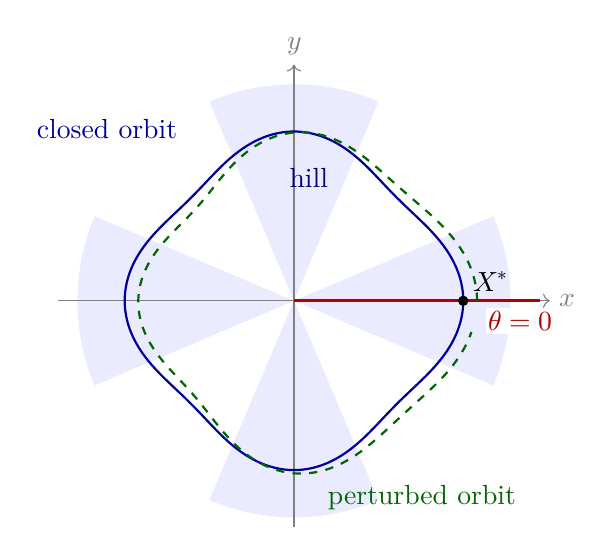
\begin{tikzpicture}[scale=1.25]
\foreach \k in {0,...,3} {
  \fill[blue!8,rotate=90*\k] (0,0) -- (-23:2.2) arc (-23:23:2.2) -- cycle;
}
\draw[->,gray] (-2.4,0) -- (2.6,0) node[right] {$x$};
\draw[->,gray] (0,-2.3) -- (0,2.4) node[above] {$y$};
\draw[very thick,red!70!black] (0,0) -- (2.5,0) node[pos=0.92,below=2pt,fill=white,inner sep=1pt] {$\theta=0$};
\draw[thick,blue!60!black,domain=0:360,samples=200,smooth,variable=\t]
  plot ({(1.6+0.12*cos(4*\t))*cos(\t)},{(1.6+0.12*cos(4*\t))*sin(\t)});
\draw[thick,green!40!black,dashed,domain=0:350,samples=200,smooth,variable=\t]
  plot ({(1.6+0.12*cos(4*\t)+0.14*cos(1.05*\t))*cos(\t)},{(1.6+0.12*cos(4*\t)+0.14*cos(1.05*\t))*sin(\t)});
\fill (1.72,0) circle (1.5pt) node[above right] {$X^*$};
\node[blue!60!black] at (-1.9,1.75) {closed orbit};
\node[green!40!black] at (1.3,-2.0) {perturbed orbit};
\node[blue!50!black] at (0.15,1.25) {hill};
\end{tikzpicture}
\caption{Section $\theta = 0$ in a 4-sector field.
The closed orbit is scalloped with the field period, farthest out in the hills, and crosses the section at the fixed
point $X^*$.
A perturbed orbit oscillates around it; the number of oscillations per turn is the tune.}
\label{fig:section}
\end{figure}

\paragraph{Crossing the section.}
The integrator does not land on $\theta = 0$.
The benchmark harness interpolates the crossing in time between steps: four-point Lagrange interpolation of the
full-step positions and momenta.
LIONS keeps momenta at half steps, so the harness forms full-step momenta by a half Boris kick of $\vect p^{\,n-1/2}$.
That is the exact inverse of the start-up, so the recorded map is conjugate to the Boris map.
The interpolation is not symplectic, and its error is $O(\Delta t^4)$.
At 1440 steps per turn it is below the finite-difference noise of the Jacobian.

\section{Closed orbit}
The closed orbit is the fixed point $T(X^*) = X^*$.
Finding it by Newton iteration on the one-turn map, and reading the focusing from the one-turn matrix, is the classic
method of cyclotron orbit codes \cite{gordon1984}.
Newton's method on $G(X) = T(X) - X$ iterates
\begin{equation}
X_{k+1} = X_k - (M_k - I)^{-1}\,\big(T(X_k)-X_k\big),\qquad M_k = \frac{\partial T}{\partial X}(X_k),
\end{equation}
with $M$ from central differences:
\begin{equation}
M_{:,j} \approx \frac{T(X+h\,e_j) - T(X-h\,e_j)}{2h}.
\end{equation}
The Newton iteration uses $h = \SI{1e-7}{m}$ on the radial block.
The Jacobian used for tunes and $\det M$ uses $h = \SI{1e-6}{m}$ in positions and $h\,p/\rho$ in momenta (the same step
as an angle $h/\rho$).
The truncation error is $O(h^2)$ and the rounding error is $O(\varepsilon_T/h)$, with $\varepsilon_T$ the noise of the
one-turn map.
A discrete one-turn map that is only piecewise smooth breaks this picture: if a probe pair $X\pm he_j$ straddles a change of
slope, the difference quotient mixes two slopes, at any $h$.

\section{Tunes from the one-turn matrix}
In uncoupled planes $M$ is block-diagonal, with $2\times2$ blocks $M_r$, $M_z$.
For a symplectic block with $|\operatorname{tr}M_u|<2$ (stable motion), $\det M_u = 1$ and the block can be written in
Twiss form (here $\alpha$, $\beta$, $\gamma$ are the Twiss parameters, not the Lorentz factors)
\begin{equation}
M_u = I\cos\mu + \begin{pmatrix}\alpha & \beta\\ -\gamma & -\alpha\end{pmatrix}\sin\mu,\qquad
\cos\mu = \tfrac12\operatorname{tr}M_u,\qquad \mu = 2\pi Q_u
\end{equation}
\cite{courant1958}.
The trace only fixes $\cos 2\pi Q$: it gives the fractional tune, folded into $[0, 0.5]$.
Its sensitivity is
\begin{equation}
\delta Q = -\frac{\delta(\operatorname{tr}M)}{4\pi\sin 2\pi Q},
\end{equation}
which diverges near $Q\in\{0, 0.5\}$.
This is why the PSI energies where $\Qr$ crosses $1.5$ are reported separately.

When $\det M_u\ne1$, the trace formula still returns a number, but it no longer is the tune of an area-preserving
oscillation; the consistent definition is then $\cos\mu = \operatorname{tr}M_u/(2\sqrt{\det M_u})$.
The benchmark harness uses $\operatorname{tr}M_u/2$.
A $\det M_u - 1$ of \GPsiLionsDetMed{} (median), as found for LIONS on the PSI map, means the formula is used outside its validity.

\section{Conditioning of the closed orbit}\label{sec:conditioning}
For an area-preserving block,
\begin{equation}
\det(M_u - I) = 2 - \operatorname{tr}M_u = 4\sin^2(\pi Q_u).
\end{equation}
A map error $\delta$ moves the fixed point by $(I-M_u)^{-1}\delta$.
In normalised coordinates $M_u$ is a rotation by $2\pi Q_u$, and $\|(I-M_u)^{-1}\| = 1/(2\sin\pi Q_u) = 1/\sqrt{\det(M_u-I)}$:
the classic $\beta/(2\sin\pi Q)$ closed-orbit sensitivity.
The sensitivity grows as $1/\sqrt{\det(M_u-I)}$, not as $1/\det(M_u-I)$.
In case B, with a fractional $\Qr$ of \BLionsQr, $\det(M_r-I) = \BCondDet$ and the amplification is about \BSens{} in
normalised units.
This near-integer amplifier (hypothesis H4) was a candidate for the case B scatter (\cref{sec:caseB}).

\section{Tunes from tracking}
A second instrument: track a particle offset by \SI{1e-4}{m} from the closed orbit for 256 turns, record the
turn-by-turn signal, apply a Hann window, and take the frequency that maximises the windowed discrete Fourier transform.
The maximum is refined by golden-section search.
Windowing and interpolating the spectrum peak gives a frequency resolution much finer than $1/N_{\rm turns}$
\cite{bartolini1996}.
On case B0 the two instruments agree within \BzeroFFTAgree.

\chapter{Verification method}\label{ch:method}

A tracking code is verified against references whose error is known, with instruments whose own error is measured.
The benchmarks follow five rules.

\section{Register before running}
Each case states its question, metrics, configuration, references and success criteria in \nolinkurl{benchmarks/DESIGN.md}
before any run.
Criteria fixed after seeing results are labelled as amendments, with the reason.
A criterion that fails stays failed in the record, even when the reason is benign.
Two examples from the record:
\begin{itemize}
\item Case A asked OPAL RK4 to converge at fourth order in the orbit radius.
It converged at fifth order, as \cref{eq:rk4-decay} shows it must.
The criterion was wrong, and it is recorded as failed, with the derivation added after the run.
\item Case H asked that the Hermite surface have value jumps below $10^{-10}$ across cell edges, probed at $\pm10^{-9}$ of a
cell.
A smooth surface changes by its gradient times the probe distance, so the test could not pass as posed.
It was replaced by a scaling test (jumps proportional to the probe distance), documented as a change made after the
result.
\end{itemize}

\section{References with a known error}
Three kinds of reference were used, from strongest to weakest:
\begin{enumerate}
\item \textbf{Closed forms.}
A uniform field (case A): circle, period, and the Boris polygon of \cref{eq:boris-radius}.
A field linear in $r$ (case B0): closed orbit from $P/|q| = |B_0|\,r\,(1-\kappa(r-r_0))$, field index $n = \kappa r/(1-\kappa(r-r_0))$,
tunes from \cref{eq:weak-tunes}.
\item \textbf{Manufactured solutions.}
FROM\_ORBIT builds a field from a prescribed family of isochronous closed orbits \cite{planche2019,planche2023}.
The orbits and the revolution frequency are then exact by construction.
Its tunes come from a geometric formula; case G1 step 1 measured them against RF-Track on a smooth interpolation of the
map (\cref{sec:caseG1}).
\item \textbf{External codes.}
FIXPO closed orbits and tunes for the PSI Ring, OPAL-cycl \cite{adelmann2019} and RF-Track
\cite{latina2023}.
Their error is not known in advance; it is bounded by comparing them with each other.
\end{enumerate}

\section{Field parity}
Codes compared on ``the same field'' must see the same field.
In the synthetic-field cases (A, B0, B2, D2), every converted field is sampled from the LIONS field evaluation itself,
so a conversion cannot add a second field model, and before each run the field of every code is compared with LIONS at
random points.
On the external maps (G1, G2) this is not possible: OPAL reads the PSI file natively and recomputes the derivatives,
and RF-Track runs on splines; there the field models differ by design and the comparison measures that.
In case B0, $B_z$ agrees within \BzeroParityBz~T and $B_x$, $B_y$ within \BzeroParityBxy~T, below the derived bound of
the LIONS chord error.
A failed parity check stops the run.
One did: the first case B2 check, written for \num{1e-13}~T on all components, failed at \num{4.9e-5}~T, and the bound
was rederived before running (\texttt{DESIGN.md}, section 14).

\section{Separate the error sources}
A tracking result mixes three errors: the field model (interpolation), the integrator (step), and the measurement
(section crossing, finite differences, Newton tolerance).
The cases are built to change one at a time:
\begin{itemize}
\item same field, different integrators and steps: B0, D2;
\item same integrator, same nodes, different interpolation: G1 step 3 (bilinear against splines, Boris fixed);
\item same field, different integrator: G2 step 2c (RF-Track on the bilinear field);
\item same code path, two implementations: the numpy Boris harness reproduces LIONS to \GValidationMax{} over one turn before it is used
for anything else.
\end{itemize}

\section{Competing hypotheses}
When a result is unexpected, the rival explanations are written down with the observation that would separate them,
and a discriminating run is registered.
\Cref{tab:evidence} shows the evidence matrix that built up for the bilinear-map noise across cases B, G1 and G2.

\begin{table}[t]
\centering\small
\caption{Evidence matrix for the noise of LIONS one-turn maps on bilinear maps.
H1: the bilinear field (kinks at cell edges). H1b: the Boris step on a kinked field. H2: a LIONS-specific defect.
H3: the finite-difference Jacobian. H4: a near-integer tune amplifying small errors.
$+$ supports, $-$ contradicts, $\cdot$ neutral.}
\label{tab:evidence}
\begin{tabular}{p{7.4cm}ccccc}
\toprule
Observation & H1 & H1b & H2 & H3 & H4\\
\midrule
B0 (bilinear exact in $B_z$): orbit order 2, $\det-1\sim10^{-9}$ & $+$ & $\cdot$ & $-$ & $-$ & $\cdot$\\
B: RF-Track on the closed-form field is clean at the same tune & $+$ & $\cdot$ & $\cdot$ & $\cdot$ & $\cdot$\\
B-gradient: OPAL spread follows $1/(2\sin\pi\Qr)$, LIONS partly & $\cdot$ & $\cdot$ & $\cdot$ & $\cdot$ & $+/-$\\
B: halving the map step does not reduce the scatter & $-$ (as $O(h^2)$) & $\cdot$ & $\cdot$ & $\cdot$ & $\cdot$\\
G1 step 3: same Boris, same nodes, spline field removes the floor & $+$ & $+$ & $\cdot$ & $\cdot$ & $\cdot$\\
G2 2b: numpy Boris on the bilinear field equals LIONS & $+$ & $+$ & $-$ & $\cdot$ & $\cdot$\\
G2 2b: $\det$ changes at most \GTwoBJacVar\,\% from $h=10^{-7}$ to $10^{-5}$ m & $\cdot$ & $\cdot$ & $\cdot$ & $-$ & $\cdot$\\
G2 2c: RF-Track on the bilinear field, $|\det-1|$ \GTwoCRatioMin{} to \GTwoCRatioMax{} times smaller & $\cdot$ & $+$ & $\cdot$ & $\cdot$ & $\cdot$\\
H: F1 (C$^1$) with Boris removes the $\det$ floor on all maps & $+$ & $+$ & $\cdot$ & $\cdot$ & $\cdot$\\
\bottomrule
\end{tabular}
\end{table}

The current best explanation is H1b: the Boris step crossing gradient jumps of a bilinear field.
H1 as first stated, an $O(h^2)$ interpolation error, failed its own prediction.
In case B, halving the azimuthal step left the scatter unchanged (ratio \BHalfDegQrRatioMin{} to
\BHalfDegQrRatioMax), where $O(h^2)$ predicts 0.25.
Kinks of any spacing (H1$'$) remain consistent with every observation.
A direct test, a Jacobian step scan with the closed orbit moved across a cell edge, has not been run.

\chapter{Benchmark results}\label{ch:results}

Each section gives the setup, the result, and the reading.
Single particles are deterministic, and each configuration was run once per code: ``one instrument'' means a single
code path measured the number.

\section{Case A: uniform field}\label{sec:caseA}
\textbf{Setup.} $B_z = \SI{1}{T}$, a \SI{1}{MeV} proton, one turn, 90 to 1440 steps per turn.
LIONS Boris, OPAL LF2 and RK4, RF-Track adaptive integrators.

\textbf{Result} (\cref{fig:caseA}).
LIONS converges at order \AlionsRadOrder{} in radius, with \AlionsRadFourteen{} at 1440 steps.
Its fitted radius equals the Boris polygon radius of \cref{eq:boris-radius} within \AlionsPolygon, and $|\vect p|$ is exact.
OPAL LF2 keeps $|\vect p|$ within \ALFTwoP; its radius is exact because its positions are chord midpoints
(\cref{sec:boris-uniform}), so only the phase discriminates, and its phase error matches the Boris closed form.
OPAL RK4 loses $|\vect p|$ by \ARkFourPThreeSixty{} per turn at 360 steps, against \ARkFourPred{} from
\cref{eq:rk4-decay}.
Its fitted radius error is \ARkFourRadThreeSixty, half of that.
This is expected if the radius decays linearly over the turn and the fit returns the mean, but it was derived after the
run.

\textbf{Reading.}
LIONS Boris behaves exactly as the analysis predicts, to rounding.
The registered criterion for RK4 (fourth order in radius) was wrong; RK4 radius and $|\vect p|$ errors are fifth order.

\begin{figure}[t]
\centering
\includegraphics[width=0.95\textwidth]{case_a}
\caption{Case A. Left: relative radius error against steps per turn, with the Boris prediction $(\omega\Delta t)^2/8$
and the RK4 amplitude decay. Right: relative error of the angle swept per step, with the Boris closed form
$1-2\arctan(\omega\Delta t/2)/\omega\Delta t\approx(\omega\Delta t)^2/12$. LIONS and OPAL LF2 overlap in phase.}
\label{fig:caseA}
\end{figure}

\section{Case B0: smooth radial gradient}\label{sec:caseB0}
\textbf{Setup.} $B_z = B_0(1-\kappa(r-r_0))$, $B_0 = \SI{-1}{T}$, $\kappa = \SI{0.5}{m^{-1}}$, $r_0 = \SI{0.15}{m}$, 1 to \SI{5}{MeV}
protons, on a bilinear map of \SI{5}{mm} by \SI{1}{\degree}.
$B_z$ is linear in $r$ and constant in $\theta$, so bilinear interpolation is exact for it.
Exact references from \cref{sec:weak}.

\textbf{Result} (\cref{fig:caseB0}).
LIONS converges at order \BzeroLionsOrderMin{} or better, with closed-orbit errors up to \BzeroLionsFourteenMax{} at
1440 steps.
Its $\Qz$ is low by up to \BzeroLionsQzErrMax.
This is consistent with the chord error of the interpolated $\partial_xB$, $\partial_yB$ (the horizontal field
follows the chord of $(\cos\theta,\sin\theta)$ between nodes), which shifts $\Qz$ by about $10^{-5}$ relative (estimate in \nolinkurl{benchmarks/DESIGN.md}, section 12).
RF-Track reaches the tolerance level.
OPAL LF2 and RK4 share an energy-dependent orbit offset, up to \BzeroOpalOffset{} relative (RK4), that is not explained; single-precision field
storage was ruled out from the source.
The Jacobian tunes and the Fourier tunes of LIONS agree within \BzeroFFTAgree.

\textbf{Reading.}
On a field without kinks in the plane, LIONS is a clean second-order code.
The orbit-error tolerance of $10^{-6}$ in the first draft is out of reach of Boris at 1440 steps, whose radius error in a
uniform field is $(\omega\Delta t)^2/8 = \AlionsRadFourteen$.
It was dropped after an exploratory LIONS run at \SI{1}{MeV} showed this, and before the registered B0 runs.

\begin{figure}[t]
\centering
\includegraphics[width=0.6\textwidth]{case_b0}
\caption{Case B0: closed-orbit radius error against the exact value, range over 1 to \SI{5}{MeV} (band) and maximum (line).}
\label{fig:caseB0}
\end{figure}

\section{Case B: 4-sector field on a bilinear map}\label{sec:caseB}
\textbf{Setup.} $B_z = B_0(1+0.3\cos4\theta)$, $B_0 = \SI{-1}{T}$, same map grid.
Report only: no pass/fail.

\textbf{Result} (\cref{fig:caseB}).
The tunes scatter with the step count, by up to \BQrSpreadMax{} in $\Qr$ over the map codes (LIONS:
\BLionsQrSpread), with no trend.
$|\det M - 1|$ ranges from \BDetMin{} to \BDetMax{} for the map codes, also without a trend.
On the closed-form field without a map, RF-Track at the same tune scatters by \BsmoothQrSpread{} in $\Qr$.
Halving the azimuthal map step does not reduce the LIONS scatter (ratio \BHalfDegQrRatioMin{} to
\BHalfDegQrRatioMax).

\textbf{Discriminating runs} (case B2, registered before running).
A radial gradient moves $\Qr$ away from 1.
Per energy, $\det(M_r - I)$ grows by \BTwoCondMin{} to \BTwoCondMax{} times (from the LIONS $\Qr$ at 1440 steps), so the
closed-orbit sensitivity $1/(2\sin\pi\Qr)$ falls by \BTwoSensMin{} to \BTwoSensMax{} (\cref{sec:conditioning}).
The orbit spread across step counts fell by \BTwoSpreadLionsMin{} to \BTwoSpreadLionsMax{} (LIONS), \BTwoSpreadLFMin{} to
\BTwoSpreadLFMax{} (OPAL LF2) and \BTwoSpreadRKMin{} to \BTwoSpreadRKMax{} (OPAL RK4).
On the closed-form field RF-Track stayed clean at the near-integer tune.

\textbf{Reading, corrected.}
The registered prediction expected the spread to fall by the full $\det(M_r-I)$ ratio, and on that basis
\nolinkurl{benchmarks/DESIGN.md} (section 15) rejected H4.
The prediction used the wrong scaling: the sensitivity goes as $1/\sqrt{\det(M_r-I)}$.
With the correct scaling, the OPAL spreads fall by amounts of the predicted size, within a factor of a few either way,
while the LIONS spread falls as predicted at one energy of five and much less at the others.
The clean RF-Track run shows that the map is the source of the errors; it says nothing about amplification, because the
errors it would amplify are tiny.
So the map is the source, and near-integer amplification (H4) is not excluded: it may add to the scatter at low
energy.

\begin{figure}[t]
\centering
\includegraphics[width=0.6\textwidth]{case_b_scatter}
\caption{Case B at \SI{1}{MeV}: fractional $\Qr$ against steps per turn.
The map codes scatter at the $10^{-3}$ level; RF-Track on the closed-form field (no map) is flat.}
\label{fig:caseB}
\end{figure}

\section{Case D2: a long-term invariant}\label{sec:caseD}
\textbf{Setup.}
In the B0 field the canonical angular momentum is an exact invariant of planar motion.
In LIONS units,
\begin{equation}
L = x p_y - y p_x + \frac{q}{m_0c}\,B_0\left(\frac{(1+\kappa r_0)\,r^2}{2} - \frac{\kappa\,r^3}{3}\right).
\end{equation}
One particle at \SI{1}{MeV}, \SI{1}{mm} off the closed orbit, \DTurns{} turns at 360 steps per turn (the largest step).
A secular change below $10^{-9}$ counts as no drift.

\textbf{Result} (\cref{tab:caseD}).
LIONS Boris and OPAL LF2 show no drift and a bounded oscillation of $L$; $|\vect p|$ is conserved to rounding.
RK4 loses $|\vect p|$ as \cref{eq:rk4-decay} predicts over \DTurns{} turns (\DRkFourPred), and $L$ drifts with it.
RF-Track drifts at the level of its tolerance accumulated over the run.

\textbf{Reading.}
On this test the Boris step behaves like a symplectic integrator: bounded oscillation, no secular drift.
That is consistent with symplectic behaviour; it is not a proof.
One field, one amplitude, planar motion.
The LIONS oscillation of $L$ is \DOscRatio{} times that of LF2; this was not analysed.

\begin{table}[h]
\centering\small
\caption{Case D2, \DTurns{} turns at 360 steps per turn.}
\label{tab:caseD}
\input{gen/tab_d2.tex}
\end{table}

\section{Case G1: manufactured solutions}\label{sec:caseG1}
\textbf{Setup.}
FROM\_ORBIT maps from the published 3-sector (H$_2^+$, three orbits from 19 to \SI{130}{MeV}) and 10-sector examples
(protons, four orbits from 932 to \SI{1630}{MeV}) of FROM\_ORBIT \cite{planche2019,planche2023}, shown in
\cref{fig:field-maps}.
The exact field is evaluated by FROM\_ORBIT's own root finding on a \thirddeg{} master grid; coarser maps are
subsets of its nodes.
\begin{itemize}
\item Step 1: RF-Track on a quintic spline of the master measures the precision of the references.
On the 3-sector map the prescribed orbits are reproduced to \GThreeRefOrbit{} and the FROM\_ORBIT geometric tunes are
good to \GThreeRefQr{} ($\Qr$) and \GThreeRefQz{} ($\Qz$); on the 10-sector map, to \GTenRefOrbit{} in orbit radius and
\GTenRefQr{} in the tunes.
The RF-Track tunes become the tune references.
\item Step 2: LIONS on bilinear maps at \thirddeg{}, \SI{1}{\degree} and \SI{4}{\degree}.
\item Step 3: the same Boris step (numpy harness, validated against LIONS) on bicubic and quintic splines of the same nodes.
\end{itemize}

\textbf{Result} (\cref{fig:G1}).
At \SI{4}{\degree} LIONS could not find the closed orbit in \GThreeFourDegFailed{} (3-sector) and \GTenFourDegFailed{}
(10-sector) configurations.
At \thirddeg{} and 1440 steps, the worst errors are:

\begin{center}\small
\begin{tabular}{lcccc}
\toprule
 & \multicolumn{2}{c}{3-sector} & \multicolumn{2}{c}{10-sector}\\
 & bilinear (LIONS) & spline (Boris) & bilinear (LIONS) & spline (Boris)\\
\midrule
$|\Delta\Qr|$ & \GThreeBilQrMax & \GThreeSplQrMax & \GTenBilQrMax & \GTenSplQrMax\\
$|\det M-1|$ & \GThreeBilDetMax & \GThreeSplDetMax & \GTenBilDetMax & \GTenSplDetMax\\
$|\Delta r_{eo}|/r$ & \GThreeBilReoMax & \GThreeSplReoMax & \GTenBilReoMax & \GTenSplReoMax\\
\bottomrule
\end{tabular}
\end{center}

With splines the errors converge at second order in orbit, turn time and tunes (closed-orbit error ratio per halving of
the step \GThreeSplOrbitRatioMin{} to \GThreeSplOrbitRatioMax{} on the 3-sector map, \GTenSplOrbitRatioMin{} to
\GTenSplOrbitRatioMax{} on the 10-sector map).
With the bilinear field the tune errors do not converge on the 3-sector map, and converge at most at first order on the
10-sector map (worst $|\Delta\Qr|$ \GTenBilQrMaxThreeSixty{} at 360 steps, \GTenBilQrMax{} at 1440); $\det M - 1$ stays
orders of magnitude above the spline values.
At 360 steps the closed-orbit errors of both are close, so there the integrator dominates.
At 1440 steps the bilinear orbit error is larger than the spline one on the 10-sector map.
On the 10-sector map at \SI{1}{\degree} (18 nodes per \SI{18}{\degree} harmonic) even the splines stop converging
cleanly.

\textbf{Reading.}
Only the interpolation changed between steps 2 and 3, so the tune excess and the $\det$ excess on these maps come with the
bilinear interpolation; \cref{tab:evidence} separates the field model from the integration across its kinks.
With splines, the isochronism error (turn time) at 1440 steps is set by the Boris step: at most \GThreeSplTurnTimeMax{}
(3-sector) and \GTenSplTurnTimeMax{} (10-sector); on the bilinear maps it is larger.
Over 500 turns at harmonic number $h_{\rm rf}$, a turn-time error of $10^{-6}$ would be an RF phase slip of order
$2\pi h_{\rm rf}\times500\times10^{-6}$~rad; this is an estimate, not simulated.

\begin{figure}[t]
\centering
\includegraphics[width=0.9\textwidth]{g1}
\caption{Case G1 at \thirddeg{}: $|\Delta\Qr|$ and $|\det M-1|$ against steps per turn.
LIONS on the bilinear map (blue) against the same Boris step on bicubic and quintic splines of the same nodes.
Bands: range over the orbits; lines: maximum.}
\label{fig:G1}
\end{figure}

\section{Case G2: PSI Ring against FIXPO}\label{sec:caseG2}
\textbf{Setup.}
The PSI Ring \SI{590}{MeV} map (8-fold, \thirddeg{}, $r$ from 1.9 to \SI{4.7}{m}) and the FIXPO equilibrium orbits
and tunes from 72 to \SI{530}{MeV}.
LIONS on the native-resolution map (1081 columns), the Boris harness on a quintic spline, RF-Track on the same spline,
and the OPAL closed-orbit finder.
All at 1440 steps per turn (RF-Track: 2880 samples), no trim coil.
At \SI{512}{MeV} OPAL returned a non-solution without an error; that energy is excluded for every code in the table.

\textbf{Result} (\cref{fig:G2}, \cref{tab:G2}).
Closed-orbit radii of every code agree with FIXPO at the level of the print resolution of the reference file
(\SI{0.1}{mm}), so the radius comparison cannot separate the codes.
The smooth-field instruments are closest to FIXPO in $\Qr$ (median \GPsiSplineQrMed{} and \GPsiRftrackQrMed), then OPAL
(\GPsiOpalQrMed), then LIONS (\GPsiLionsQrMed).
On the bilinear map the radial tune is defined only roughly: the case H harness with the same node data (F0, Boris,
$\operatorname{atan2}$ azimuth, its own Newton solution) agrees with LIONS at some energies and differs several-fold at
others, giving a median of \HFixpoBilQrMed{} against FIXPO (\cref{sec:caseH}).
LIONS has $|\det M - 1|$ of \GPsiLionsDetMed{} (median), up to \GPsiLionsDetMax.
All these tunes come from the one-turn Jacobian.
Tracked over many turns, LIONS on the same field is within \GThreeFiveFixMax{} of FIXPO at \SI{5}{mm} (\cref{sec:caseG3}), so the LIONS line of \cref{tab:G2} does not measure the betatron frequency of a beam.

\begin{table}[h]
\centering\small
\caption{Case G2: absolute errors against FIXPO, median / maximum over the interior energies of the step-3 grid
(92 to \SI{492}{MeV}, without the 386 to \SI{430}{MeV} band and \SI{512}{MeV}).}
\label{tab:G2}
\input{gen/tab_g2.tex}
\end{table}

\begin{figure}[t]
\centering
\includegraphics[width=0.8\textwidth]{g2_tunes}
\caption{Case G2: tune errors against FIXPO over the energy range.
Grey band: $\Qr$ near 1.5, where the trace formula is ill-conditioned.}
\label{fig:G2}
\end{figure}

\textbf{Discriminating runs} (steps 2b and 2c, \cref{tab:G2det}).
The numpy Boris on the bilinear field reproduces LIONS, so the effect is not a LIONS defect (H2 rejected).
The determinant barely moves with the Jacobian step, which argues against a finite-difference artefact (H3) without
excluding it (\cref{ch:orbits}, \cref{tab:evidence}).
The effect is in the radial block only; the vertical block is clean.
RF-Track (adaptive) on the same bilinear field gives a $|\det M_r - 1|$ \GTwoCRatioMin{} to \GTwoCRatioMax{} times
smaller; the registered reading threshold ($10^{-3}$) was met at one energy of three.
Since the exact flow preserves area on any continuous field (\cref{ch:integrators}), the $\det$ excess must come from
the discretisation.
This is consistent with H1b, fixed-step integration across gradient jumps; case H shows that fixed-step RK4 has the
same excess (\cref{sec:caseH}).

\begin{table}[h]
\centering\small
\caption{Case G2: $\det M_r - 1$ of the radial block at three energies, Jacobian step \SI{1e-6}{m}.}
\label{tab:G2det}
\input{gen/tab_g2_det.tex}
\end{table}

\paragraph{A criterion that could not fail.}
The registered G2 criterion was $|L-F|\le|O-F|+|L-S|$ per metric and energy, with $L$ LIONS, $F$ FIXPO, $O$ OPAL and $S$
the spline tracker.
By the triangle inequality $|L-F|\le|L-S|+|S-F|$, so whenever the spline tracker is at least as close to FIXPO as OPAL,
the criterion holds whatever LIONS does.
It passed for $\Qr$ while LIONS was \GPsiLionsOverOpal{} times further from FIXPO than OPAL (median).
The informative comparison is \cref{tab:G2}.
The criterion was proposed by this analysis, and the record says so.

\section{Case G3: OPALX and the step phase}\label{sec:caseG3}
\textbf{Question} (registered before running).
Does OPALX 1.0.0 \cite{opalx2026} reproduce OPAL 2024.1 and FIXPO on the PSI map, and does a third, independent tracker on the same bilinear field show the $\det M_r$ excess?
OPALX interpolates $B_z$ bilinearly on the same nodes.
Its closed-orbit command writes the Jacobian; no trim coil, 1440 steps, the G2 step 3 energies.
The installation reproduces its own regression test on this map within its tolerances.

\textbf{Result} (\cref{tab:G3,tab:G3det}).
No run failed.
The excess is not specific to LIONS: OPALX Boris has a median $|\det M_r-1|$ of \GThreeBorisDet{}, RK4 \GThreeBorisOverRk{} times less, and the fixed-step eighth-order DOP853 \GThreeDopOverRk{} times more than RK4.
No integrator shows its order: the values are not monotonic in the step count and they change sign.
The OPALX manual reports the same behaviour on this map at 46080 steps per turn, with a radial modulus off unity by $10^{-4}$ to $10^{-3}$, and names the piecewise interpolation as an unconfirmed candidate \cite{opalx2026}.
OPALX Boris $\det M_r$ moves at most \GThreeFdVar\,\% with the derivative step from $10^{-7}$ to $10^{-5}$.

\begin{table}[h]
\centering\small
\caption{Case G3: OPALX against FIXPO, median / maximum over the energies of \cref{tab:G2}, Jacobian tunes, 1440 steps.
$|\operatorname{tr}M_r/2|>1$ at several energies, where the tune is clipped to 0.5; the maxima include these.}
\label{tab:G3}
\input{gen/tab_g3.tex}
\end{table}

\begin{table}[h]
\centering\small
\caption{Case G3: OPALX $\det M_r - 1$ against steps per turn.}
\label{tab:G3det}
\input{gen/tab_g3_det.tex}
\end{table}

One registered prediction failed.
OPALX minus OPAL 2024.1 in $\Qr$ has a median of \GThreeOpalQrMin{} to \GThreeOpalQrMax{}, where below $10^{-3}$ was predicted, because the premise of a shared field model does not hold for tunes.
From its source, the OPAL finder integrates the linearised equations with the interpolated $\partial_rB$ and $\partial_\theta B$ channels, so it sees a continuous gradient.
OPALX differentiates the tracked map, which sees the gradient jumps of bilinear $B_z$.
This explanation is read from the sources, not tested.

\paragraph{The same field in two codes.}
LIONS and OPALX Boris have the same magnitude of $\det M_r-1$ but not the same value: the correlation over the 24 energies is \GThreeCorr.
OPALX also subdivides steps at sector edges.
So $\det M_r$ is a property of the discrete map and of where its steps fall, not a stable property of the field.

\paragraph{Tracked tunes.}
OPALX spectral tunes (a ray \SI{5}{mm} off, RK4, 100 turns) lie within \GThreeSpecQrMax{} of FIXPO in $\Qr$ at \GThreeSpecN{} of \GThreeSpecN{} energies (bin \num{2.5e-3}), the half-integer band included.
A registered run then measured LIONS itself: launch at amplitude $a$ in $r$ and $z$ from the code's own closed orbit, 100 turns, tune from the turn-by-turn signal (\cref{tab:G3amp}, \cref{fig:G3}).
LIONS is within \GThreeFiveSplMax{} of the spline tracker at \SI{5}{mm}, \GThreeOneSplMax{} at \SI{1}{mm} and \GThreeTenthSplMax{} at \SI{0.1}{mm}.
At \SI{0.01}{mm} it is more than 0.1 off at \GThreeSmallOff{} of \GThreeSmallN{} energies.
The Hermite option stays close at every amplitude (median against FIXPO \GThreeHermQrMed{} in $\Qr$ and \GThreeHermQzMed{} in $\Qz$; spline \GThreeSplQzMed{} and default \GThreeLionsQzMed{} in $\Qz$).

\begin{table}[h]
\centering\small
\caption{Case G3 step 2: tracked $|\Qr-\Qr^{\rm FIXPO}|$, median / maximum over 22 energies outside the band, and the ratio of the rms radial amplitude over the last and first ten of 100 turns.
Baseline of that ratio on the smooth models: \GThreeArBaseMin{} to \GThreeArBaseMax{} (beating at low tune).}
\label{tab:G3amp}
\input{gen/tab_g3_amp.tex}
\end{table}

\begin{figure}[t]
\centering
\includegraphics[width=\textwidth]{g3_phase}
\caption{Left: radial tune error of LIONS on the PSI map, from the one-turn Jacobian and from tracking.
Grey band: $\Qr$ near 1.5.
Right: distance from the closed orbit at \SI{292}{MeV}, in units of the launch amplitude, at the nominal step and on a commensurate turn.}
\label{fig:G3}
\end{figure}

\paragraph{The step phase.}
A \SI{0.01}{mm} oscillation does not grow as $\det M_r$ implies: its amplitude ratio is at most \GThreeSmallArMax, against up to \GThreeSmallPred{} from $(\det M_r)^{45}$.
The registered reading of that failure was that the Jacobian was suspect again, so the Jacobian was tested directly (step 2b, 30 turns, \SIrange{1e-7}{1e-4}{m}).
$M$ predicts the first return within \GThreeOneTurnMin{} to \GThreeOneTurnMax{} at $a=\SI{1e-7}{m}$.
At the second return the prediction fails by order 1, which also missed the registered prediction.
From then on the distance to the closed orbit no longer depends on $a$: at \SI{152}{MeV} and turn 5 it is \GThreeJitterA{}~m from $a=\SI{1e-7}{m}$ and \GThreeJitterB{}~m from $a=\SI{1e-6}{m}$.

Hypothesis S: the turn time is not an integer number of steps, so each turn starts at another step phase and is another map.
At the nominal step these energies miss a commensurate turn by \GThreeSlipMin{} to \GThreeSlipMax{} of a step per turn (turn time between the first two crossings, G2 step 2).
Test (step 2c): adjust the step until one turn is exactly 1440 steps, and repeat.
At turn 2 the deviation falls to \GThreeComTwoMin{} to \GThreeComTwoMax, and the growth no longer depends on $a$ and tracks $M^n$ (\cref{fig:G3}, right).
At \SI{292}{MeV} a launch grows by \GThreeComGrow{} in 20 turns, against \GThreeComGrowPred{} from $M^n$.
This refutes the rival that the second-return failure does not depend on the step phase.
It misses the registered threshold ($10^{-2}$ through turn 10): the deviation at turn 10 is \GThreeComTenMin{} to \GThreeComTenMax, not explained.

\begin{reading}
This reading is a proposal.
On a bilinear field, the one-turn map depends on the step phase at the section.
The Newton solution and $M$ of cases G2, H and G3 are correct for one phase.
Over many turns the orbit moves among these maps.
Then:
(1) tracked tunes are right, with a median of \GThreeTenthFixMed{} against FIXPO at \SI{0.1}{mm};
(2) below about \SI{0.1}{mm} the betatron signal is lost in a jitter of tens of micrometres;
(3) amplitudes are not reliable: the radial amplitude at \num{0.1} and \SI{1}{mm} changes by \GThreeArMin{} to \GThreeArMax{} times in 100 turns on a coasting orbit;
(4) a deliberately commensurate step makes the growth exponential;
(5) the Hermite field removes all of this in the runs above.
That each phase has its own fixed point is inferred, not measured.
Beam size and emittance over longer runs, on a bunch and with acceleration have not been measured.
\end{reading}

\chapter{Field-model options for LIONS}\label{ch:options}

\section{Case H: which option removes the excess, at what cost}\label{sec:caseH}
\textbf{Question.}
Which opt-in additions to LIONS remove the G1 and G2 excess errors, and at what cost per particle-step?
The bilinear field and the Boris step stay the default, and the Fortran bit-identity of the default path is kept.

\textbf{Design} (registered before running).
Four field models on the same node data (F0 bilinear, F1 bicubic Hermite, F2 cubic and F3 quintic splines;
\cref{ch:interpolation}) and two integrators: Boris, and RK4 with a fixed step.
Three step counts (720, 1440, 2880 per turn), and three maps: 3-sector and 10-sector FROM\_ORBIT at \thirddeg{} and
\SI{1}{\degree}, and the PSI Ring.
Decision target, fixed before the run: $|\Delta\Qr|$, $|\Delta\Qz|$ and $|\det M - 1|$ all at most $10^{-4}$ on every orbit
or energy of a map.
The validation came first.
F1 reproduces node values and derivatives to \HFOneNodes, and RK4 shows fourth order from 360 steps per turn.

\textbf{Result} (\cref{fig:H}, \cref{tab:Hdecision,tab:Hcost}).
\begin{itemize}
\item F0 never meets the target, with either integrator.
RK4 does not fix it: on the 10-sector and PSI maps its worst $|\det M - 1|$ at 1440 steps is \HFzeroRkDetMin{} to
\HFzeroRkDetMax, \HBorisOverRkMin{} to \HBorisOverRkMax{} times below Boris on all maps.
Both decrease with the step count, slowly: fixed-step integration across the gradient jumps limits every integrator.
\item F1 with Boris meets the target wherever any option does, at the lowest cost per turn, on the FROM\_ORBIT maps:
720 steps on the 3-sector map, 2880 on the 10-sector map at \thirddeg{}.
\item No option meets it on the 10-sector map at \SI{1}{\degree}: too few nodes per harmonic period
(\cref{ch:interpolation}).
\item On the PSI map the reference is RF-Track on F3, which favours F3; only F3 meets the target against it.
Against FIXPO, the external reference, F1 with Boris at 1440 steps is the closest model: median $|\Delta\Qr|$
\HFixpoHermQrMed{} and $|\Delta\Qz|$ \HFixpoHermQzMed, against \HFixpoBilQrMed{} and \HFixpoBilQzMed{} for F0,
\HFixpoCubQrMed{} and \HFixpoCubQzMed{} for F2, \HFixpoQuinQrMed{} and \HFixpoQuinQzMed{} for F3.
FIXPO's own interpolation is unknown; that F1 shares its use of the file derivatives is a hypothesis.
\end{itemize}

\begin{figure}[t]
\centering
\includegraphics[width=\textwidth]{h_matrix}
\caption{Case H: worst error over orbits or energies (largest of $|\Delta\Qr|$, $|\Delta\Qz|$, $|\det M-1|$) against
steps per turn, for each field model and integrator.
Dotted line: decision target $10^{-4}$.
PSI: reference RF-Track on F3; the 386 to \SI{430}{MeV} band is excluded.}
\label{fig:H}
\end{figure}

\begin{table}[h]
\centering\small
\caption{Case H: smallest step count per turn (of 720, 1440, 2880) meeting the decision target; -- means none.
B: Boris, RK: RK4.}
\label{tab:Hdecision}
\input{gen/tab_h_decision.tex}
\end{table}

\begin{table}[h]
\centering\small
\caption{Case H: cost per particle-step in the numpy harness, $10^5$ particles, PSI map, Apple M3 CPU (ratio to F0 with
Boris).
LIONS itself costs \HLionsCost{} times the harness F0, so the harness cost is representative.}
\label{tab:Hcost}
\input{gen/tab_h_cost.tex}
\end{table}

\section{F1 in LIONS}
F1 is in LIONS as the deck option \texttt{interpolation=hermite} (API: \texttt{Deck.field\_interpolation}).
LIONS derives the Hermite slopes from its own map: $\partial_rB$ and $\partial_\theta B$ from $\partial_xB$, $\partial_yB$, and the
cross derivative as in F1.
So it needs no new input file.
The Fortran code ignores the option token, which is checked by a test.

Validation against the harness: one turn agrees within \HPhaseTwoOneTurn{} relative.
Closed orbits, turn times and $\Qz$ agree to rounding.
$\Qr$ and $\det M - 1$ differ by up to \HPhaseTwoJacMax.
The registered tolerance was $10^{-9}$, so the validation failed as written.
The residual is attributed to the finite-difference Jacobian acting on the remaining rounding noise (not tested), and
it is \HTargetRatio{} or more times below the decision target.
The cost is \HPhaseTwoCostRatio{} times the default on the PSI map at $10^5$ particles.

The first implementation took the azimuth from $\arccos$ (\cref{sec:azimuth}).
Its Jacobian differed from the harness by an amount that grew as $1/h$ with the probe step $h$.
That is the signature of non-smooth noise in the one-turn map, not of a field difference.
Taking $\theta$ from $\operatorname{atan2}$ removed most of it.

\section{The \texttt{azimuth=atan2} option}
The same change is available for the default bilinear path, as \texttt{azimuth=atan2}.
\Cref{tab:Hazimuth} compares the radial Jacobian of LIONS with that of the numpy bilinear tracker (which uses
$\operatorname{atan2}$).

\begin{table}[h]
\centering\small
\caption{Maximum $|\Delta M_{rr}|$ between LIONS bilinear and the numpy bilinear tracker, for three Jacobian steps.}
\label{tab:Hazimuth}
\input{gen/tab_h_azimuth.tex}
\end{table}

The registered criterion, a tenfold reduction at $h = \SI{1e-6}{m}$, was not met on either map.
On the 10-sector map at $h = \SI{1e-7}{m}$ the noise even grew.
The working hypothesis, not tested, is that the bilinear one-turn map has a second noise source: it is only piecewise
smooth, so probes that straddle a cell edge mix two slopes.
On the C$^1$ Hermite field the same azimuth change worked, which fits this hypothesis.

\section{What to use}
\begin{itemize}
\item For tune or Jacobian work on measured maps: \texttt{interpolation=hermite}.
Its effect on autograd gradients has not been measured: the PyTorch port is bilinear only.
It lowers $|\det M-1|$ by \HDetRatioMin{} to \HDetRatioMax{} times at 1440 steps, for \HCostHerm{} times the cost of
the default; on the PSI map it still leaves \HFoneDetPsi{} at 1440 steps and \HFoneDetPsiTwoEightEighty{} at 2880 steps, while the
tunes do not meet the target against the F3 reference at any step count.
\item Check the node density per harmonic period of the map (\cref{ch:interpolation}) before trusting any interpolation.
\item The default stays for reproducing Fortran results.
\end{itemize}

\chapter{Differentiable tracking}\label{ch:differentiable}

\section{Why gradients}
Calibrating a model on machine data means fitting a few parameters (field scale, dee voltages, phases, the initial beam)
to measured quantities (probe currents, phase, extracted energy).
With gradients of the tracked observables with respect to these parameters, the fit can use gradient-based optimisers.
With $10^5$ particles, the forward model can also be fast enough for many evaluations.
Differentiable beam dynamics codes exist for linear accelerators and transfer lines \cite{kaiser2024}.
Cases E and E2 ask whether the LIONS core can join them.

\section{Reverse-mode automatic differentiation}
A tracking run is a composition $X_N = \Phi_N\circ\cdots\circ\Phi_1(X_0;\lambda)$.
Reverse mode computes $\partial f(X_N)/\partial\lambda$ for a scalar $f$ in one backward sweep, at a cost of a few forward
passes, whatever the number of parameters.
The price is memory: the backward sweep needs the intermediate states of all $N$ steps.
Checkpointing stores only every $\sqrt N$-th state and recomputes each segment during the backward sweep.
In principle memory then grows as $O(\sqrt N)$ for one extra forward pass \cite{chen2016}; recursive schemes reach
logarithmic growth \cite{griewank2000}.

\section{Case E: the port and its gradients}
The LIONS bilinear field and Boris push were ported to PyTorch \cite{paszke2019} in float64.
The port reproduces LIONS positions and momenta at every step of one turn within \EPortMax{} relative.
Gradients of $r$, $p_r$ and the phase with respect to the map scale $s$, $r_0$ and $p_{r0}$ were compared with central finite
differences (\cref{tab:Egrad}).

\begin{table}[h]
\centering\small
\caption{Case E: maximum relative difference between autograd and central finite differences at the registered steps
($10^{-6}$ relative for $s$, \SI{1e-7}{m} for $r_0$, $10^{-7}$ for $p_{r0}$).}
\label{tab:Egrad}
\input{gen/tab_e_grad.tex}
\end{table}

\begin{itemize}
\item B0, the smooth field, passes the $10^{-6}$ criterion.
\item A, the uniform field, fails on \EAFailCount{} entries.
The largest are $\partial\phi/\partial p_{r0}$ at both step counts and $\partial\phi/\partial r_0$ at 3600 steps.
These derivatives are small: in a uniform field, at fixed $|\vect p|$, the revolution period does not depend on $r_0$ or
$p_{r0}$, while the finite-difference reference carries a rounding error that grows with the phase (about $2\pi$ per
turn): there the finite difference is the noisy side.
The other failures are at most \EAFailOtherMax{} and were not analysed.
\item B, the bilinear 4-sector map, is the instructive case (\cref{fig:Efd}).
At 3600 steps the disagreement reaches \ESweepLargeH{} at $h = 10^{-4}$, falls to \ESweepSmallH{} at $h = 10^{-8}$, and
rises again at $h = 10^{-9}$ (\ESweepTinyH) from rounding.
(The summary of this sweep and of the case A failures in \nolinkurl{benchmarks/DESIGN.md}, section 19, does not match
the table; the numbers here are from the table.)
Example: $\partial r/\partial s = \EExampleAutograd$ from autograd, against \EExampleFD{} from finite differences at
$h = 10^{-6}$.
\end{itemize}

\begin{figure}[t]
\centering
\includegraphics[width=0.6\textwidth]{case_e_fd}
\caption{Case E: worst disagreement between autograd and central finite differences against the finite-difference step,
at 3600 steps (10 turns).
The bilinear map (case B) agrees only near $h=10^{-8}$; on the smooth field (B0) the disagreement stays at the
finite-difference error level (truncation at large $h$, rounding at small $h$).}
\label{fig:Efd}
\end{figure}

\begin{reading}
Autograd returns the derivative of the discrete map at the point.
On a bilinear map the discrete map is only piecewise $C^1$: its derivative jumps whenever a step point crosses a cell
edge.
A finite difference with a step larger than the spacing of these jumps averages over them.
For an optimiser this means the local gradient and the gradient over a finite parameter change differ: after ten turns,
by up to \ESweepLargeH{} for a relative change of $10^{-4}$ of the map scale $s$.
A $C^1$ field (F1) removes the jumps; whether it closes the gap for gradients has not been measured.
\end{reading}

\paragraph{Memory and time.}
Without checkpointing the autograd graph costs about \EKBPerStep~kB per step for one particle (from the $10^3$ and $10^4$
step runs), which \nolinkurl{benchmarks/DESIGN.md} (section 19) attributes to about 60 small operations per step.
The measurements (\cref{tab:Ecost}) do not follow the textbook picture.
Checkpointing reduces memory only with $10^3$ particles; with one particle it uses more.
It costs \ECkptTimeMin{} to \ECkptTimeMax{} times the time, not about two.
At $10^5$ steps it still needs several GB above the imports, far more than $\sqrt N$ stored states.
The cause was not investigated.

\begin{table}[h]
\centering\small
\caption{Case E: forward plus backward, eager PyTorch on the M3 CPU (peak RSS includes the Python and PyTorch imports).
``skipped'': extrapolated memory above half the RAM.}
\label{tab:Ecost}
\input{gen/tab_e_cost.tex}
\end{table}

\section{Case E2: throughput}
\textbf{Question} (registered before running): can a compiled PyTorch step beat plain LIONS throughput by 10 times?
This is the go criterion for building a differentiable backend.

\textbf{Result} (\cref{fig:E2}, \cref{tab:E2}).
Compiled float64 reaches \EtwoRatioH{} times plain LIONS at $10^5$ particles on an H100 (\EtwoBestH{} particle-steps per
second), \EtwoRatioA{} times on an A100, and \EtwoRatioM{} times on the M3 CPU.
At $10^3$ particles no device reaches 10.
float32 gives no speed gain on the GPUs and loses accuracy: up to \EtwoGpuFloatThirtyTwoR{} relative in $r$ after ten
turns.
GPU float64 agrees with CPU float64 within \EtwoGpuFloatSixtyFourR.

\begin{table}[h]
\centering\small
\caption{Case E2: forward throughput relative to plain LIONS on the same node, and wall time of compiled float64
forward plus backward at $10^3$ particles (3600 steps).}
\label{tab:E2}
\input{gen/tab_e2.tex}
\end{table}

\begin{figure}[t]
\centering
\includegraphics[width=0.65\textwidth]{case_e2}
\caption{Case E2: forward particle-steps per second against particle count, best float64 variant per device
(MPS: float32 only).
Dashed: plain LIONS on the CPU of the same node.}
\label{fig:E2}
\end{figure}

\begin{reading}
The go criterion is met at $10^5$ particles, on the GPUs and on the M3 CPU.
On the A100 the wall time changes from \EtwoAWallOne{}~s to \EtwoAWallMax{}~s between 1 and $10^5$ particles, so the run is launch-bound and $10^5$ is not the
ceiling.
Small-batch gradients are faster on the CPU.
\end{reading}

\section{Before trusting a calibrated model}
A model fitted on machine data inherits every omission of the simulator.
LIONS does not model space charge, a full 3D field map, misalignments of the dees or the central-region electrodes,
field drifts and hysteresis, or RF amplitude and phase noise.
A parameter fit will absorb these effects into the parameters it has.
Fitted values are therefore effective parameters until they are checked on held-out operating conditions.

\chapter{Open questions}\label{ch:open}

\section{Not run}
\begin{itemize}
\item \textbf{CIME.}
The CIME field map is not available to the benchmarks yet.
The node density per harmonic period of the CIME map, and the size of the bilinear excess on it, are therefore unknown.
Case C (acceleration through the dees) does not need it, but waits for a check of the RF time convention of each
code on a one-gap test.
\item \textbf{Extraction (case F).}
The CIME deck has one electrostatic deflector and no transfer-line element, so there is nothing after extraction to
compare between LIONS, Xsuite and Cheetah yet.
\end{itemize}

\section{Untested hypotheses}
\begin{itemize}
\item \textbf{Kink noise on the bilinear path.}
The bilinear one-turn map is only piecewise smooth, and probes that straddle a cell edge mix two slopes.
Test: a Jacobian step scan with the closed orbit moved across a cell edge.
\item \textbf{Residual on RF-Track with the bilinear field.}
RF-Track on the bilinear PSI field still leaves $|\det M_r - 1|$ up to \GTwoCRfMax{} (\cref{tab:G2det}).
Adaptive Runge--Kutta also loses order at gradient jumps, and the section crossing adds its own error.
These were not separated.
\item \textbf{OPAL offsets.}
In B0, OPAL has an energy-dependent closed-orbit offset of order $10^{-8}$ shared by LF2 and RK4.
In A, OPAL RK4 has a phase error floor near \ARkFourPhaseFloor.
Neither is explained.
\item \textbf{Gradients on F1.}
Whether the Hermite field closes the gap between autograd and finite differences on measured maps has not been measured.
\end{itemize}

\section{Physics questions for the LIONS authors}
Two behaviours were found while porting and left unchanged pending a decision:
\begin{itemize}
\item A difference between the codes: the Python port adds a vertical bunch spread for \texttt{espace='6d'}, while the
Fortran does so only for \texttt{'3d'} (\texttt{lions\_2.0\_ep.f90}, line 498).
\item Shared by both codes: the correlation code indexes the mass array by family number.
This is wrong for families after the first.
\end{itemize}

\section{Lessons}
\begin{enumerate}
\item The field smoothness sets the error level more than the integrator does.
On the bilinear maps of case H, neither Boris nor RK4 meets the $10^{-4}$ target at any step count up to 2880 per turn
(\cref{tab:Hdecision}).
A $C^1$ interpolation at \HCostHerm{} times the cost lowers $|\det M-1|$ by \HDetRatioMin{} to \HDetRatioMax{} times.
\item Count nodes per harmonic period, not degrees.
\item Fixed-step integration across gradient jumps breaks area preservation of the one-turn map by orders of magnitude
more than on a smooth field, with Boris and with RK4.
\item Every convention (units, signs, direction, reference azimuth) should be settled by a two-reading run.
\item A criterion built by the analysis that it judges can be tautological.
Write the triangle inequality down before using one.
\end{enumerate}


\appendix
\chapter{Provenance}\label{app:provenance}
Figures, tables and numbers are generated by \nolinkurl{docs/lecture/figures.py} at code version \CodeVersion{} from the
following tables (results stay at the sites and on the analysis laptop; they are not in git).
The design note \nolinkurl{benchmarks/DESIGN.md} holds the registered specifications and amendments quoted here.

\begin{center}\scriptsize\input{gen/sources.tex}\end{center}

\bibliographystyle{unsrtnat}
\bibliography{references}
\end{document}
